\subsection{Описание предметной области}
\label{subsections:DomainModel}

Далее рассматривается структура информационной модели.
В связи с тем, что в качестве целевого формата был выбран  формат Revit,
дальнейшее описание предметной области будет в первую очередь
соответствовать стандартам Autodesk Revit.
Различия с другими форматами, например Industry Foundation Classes (IFC-формат),%
\cite{BuildingSmartIFC}
рассматриваться не будут.

\begin{figure}[ht]
    \centering
    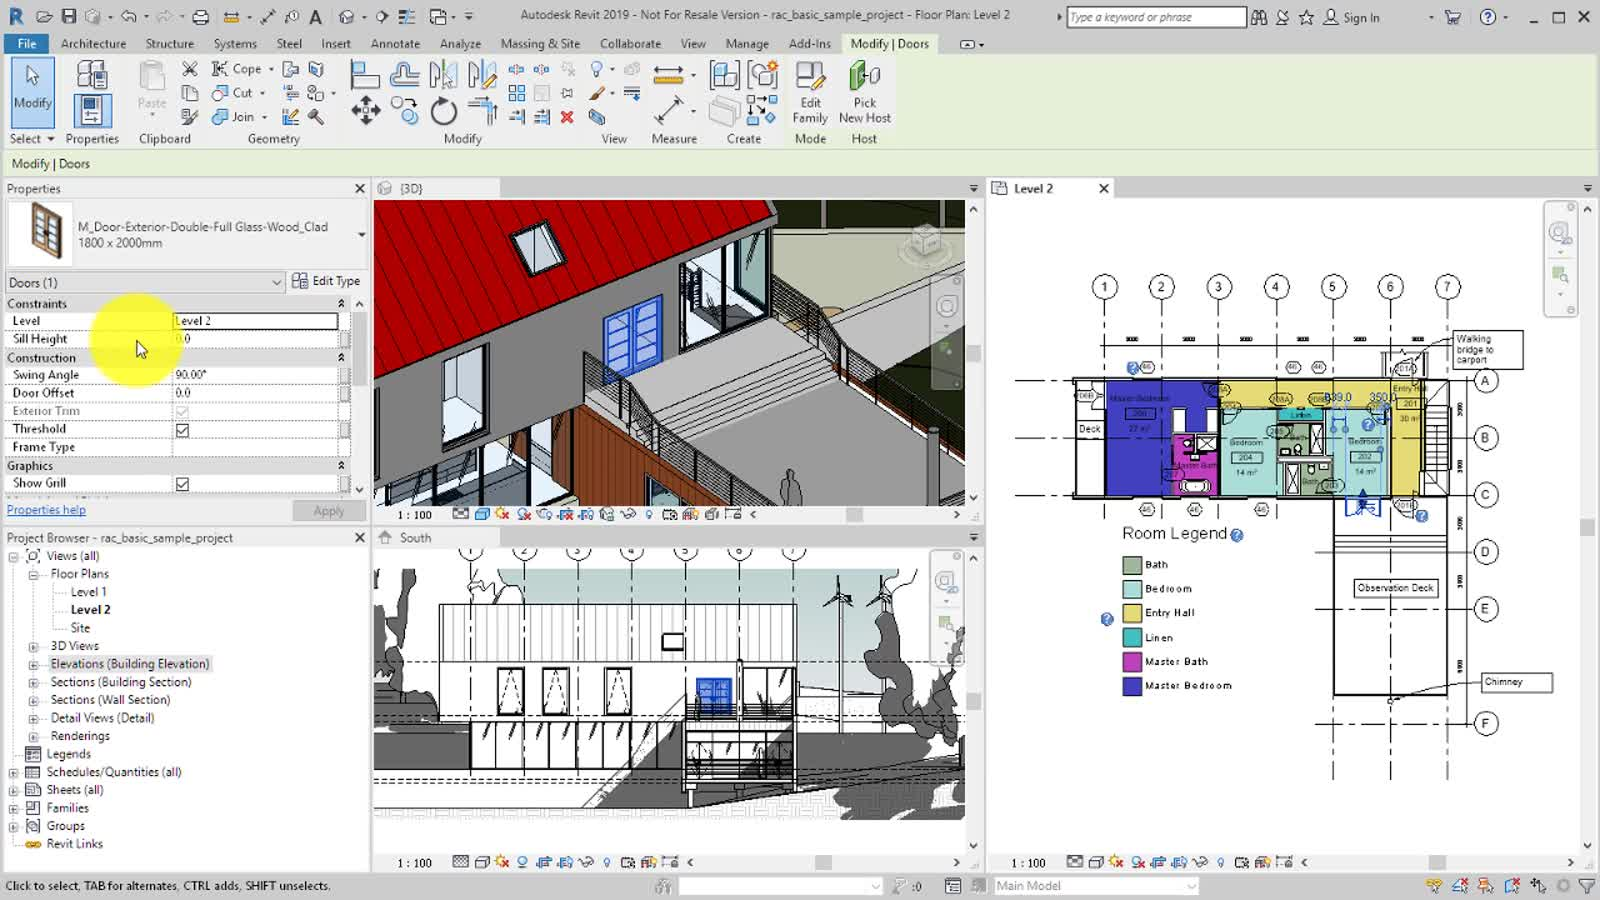
\includegraphics[width=0.9\textwidth, frame]{images/Revit-interface.jpg}
    \caption{Интерфейс редактора Revit.%
    \cite{DocRevit}}
    \label{figure:RevitInterface}
\end{figure}

Для хранения данных Revit использует специальный проприетарные форматы RVT, RFA и RTE.
Для отображения данных модели в виртуальной среде необходимо
преобразовывать их в форматы трехмерной графики, например OBJ или FBX.

\paragraph{Элементы информационной модели}

Каждая сущность в проекте информационной модели называется элементом.
Revit использует 3 типа элементов в проектах:
элементы модели, опорные элементы и элементы, относящиеся к представлению.
Элементы в Revit также часто называются семействами.
Семейство содержит геометрическое определение элемента и
параметры, используемые элементом.
Каждый экземпляр элемента определяется и контролируется семейством.%
\cite{DocRevit}
Для создания визуализации нас в первую очередь интересуют
именно элементы модели.

\begin{figure}[ht]
    \centering
    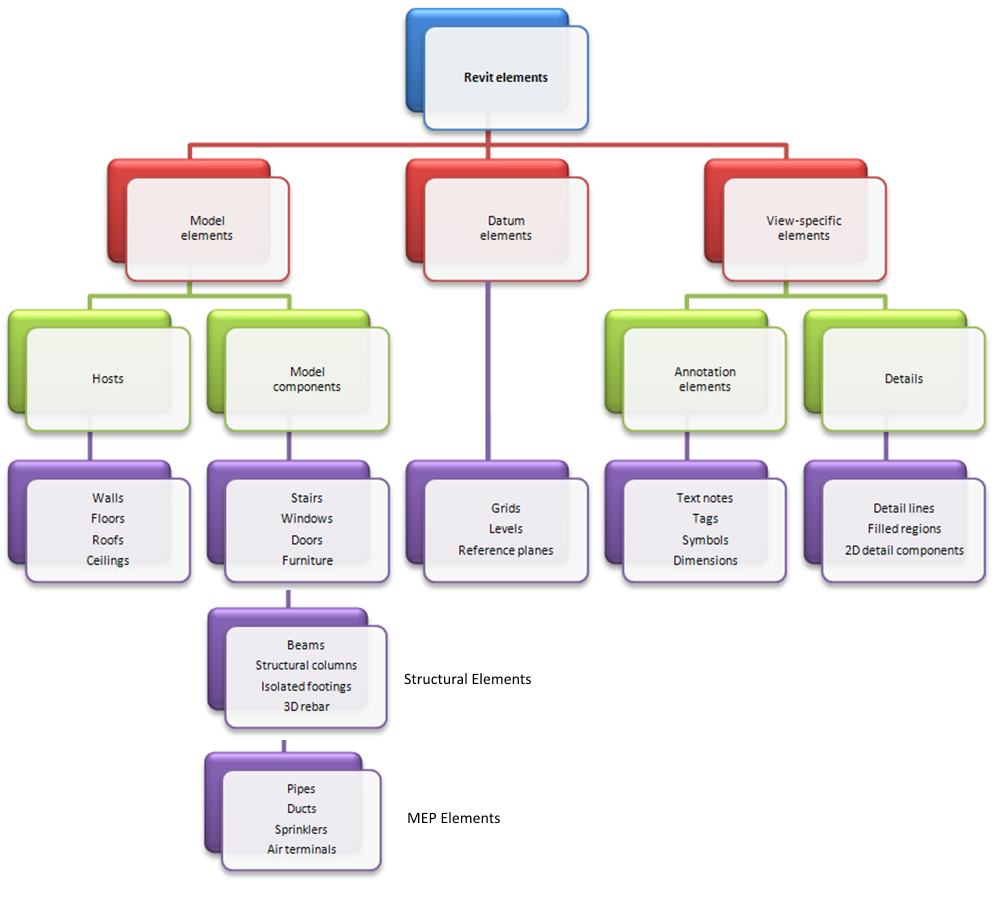
\includegraphics[width=0.9\textwidth]{images/Revit-elements.png}
    \caption{Элементы информационной модели.%
    \cite{DocRevit}}
    \label{figure:RevitElements}
\end{figure}

\begin{itemize}
    \item {
        Элементы модели.

        Элементы модели представляют фактическую трехмерную геометрию здания,
        например стены, окна, двери, пандусы,
        воздуховоды и электрические панели.
        Элементы модели делятся на хосты и компоненты модели.
        Хостами обычно являются элементы,
        которые возводятся непосредственно на строительной площадке,
        например стены и потолки.
        Компонентами модели являются все остальные типы элементов модели.
    }
    \item {
        Опорные элементы.

        Опорные элементы помогают определить контекст проекта.
        К ним относятся опорные плоскости, уровни и сетки.
    }
    \item {
        Элементы представления.

        Элементы представления это элементы,
        отображаемые только в каком-то определенном режиме представления проекта.
        Они помогают описывать или документировать модель.
    }
\end{itemize}

\paragraph{Свойства элементов}

Каждый размещаемый элемент является экземпляром семейства.
Элементы имеют 2 набора свойств, управляющих их внешним видом и поведением:
свойства типа и свойства экземпляра.%
\cite{DocRevit}

\begin{itemize}
    \item {
        Свойства типа.

        Один и тот же набор свойств типа является общим для всех элементов семейства,
        и каждое свойство имеет одинаковое значение для всех экземпляров определенного типа семейства.
        Изменение значения свойства типа влияет на все текущие и будущие экземпляры этого семейства.
    }
    \item {
        Свойства экземпляра.

        Общий набор свойств экземпляра также применяется ко всем элементам,
        принадлежащим к определенному типу семейства,
        но значения этих свойств могут различаться.
        Например, размеры окна являются свойствами типа,
        а его высота расположения над уровнем пола является свойством экземпляра.
    }
\end{itemize}
